% ============================================================================
% FreeGSNO model diagram  ---  v2 (faithful to the original img/model.png notation)
% Regenerate:  pdflatex -output-directory=img img/model_v2.tex   (from repo root)
% ============================================================================
\documentclass[border=8pt]{standalone}
\usepackage{mathptmx}
\usepackage{amsmath,amssymb}
\usepackage{tikz}
\usetikzlibrary{arrows.meta,positioning,fit,backgrounds,calc,decorations.pathreplacing}

\definecolor{nvy}{RGB}{37,78,145}

\begin{document}
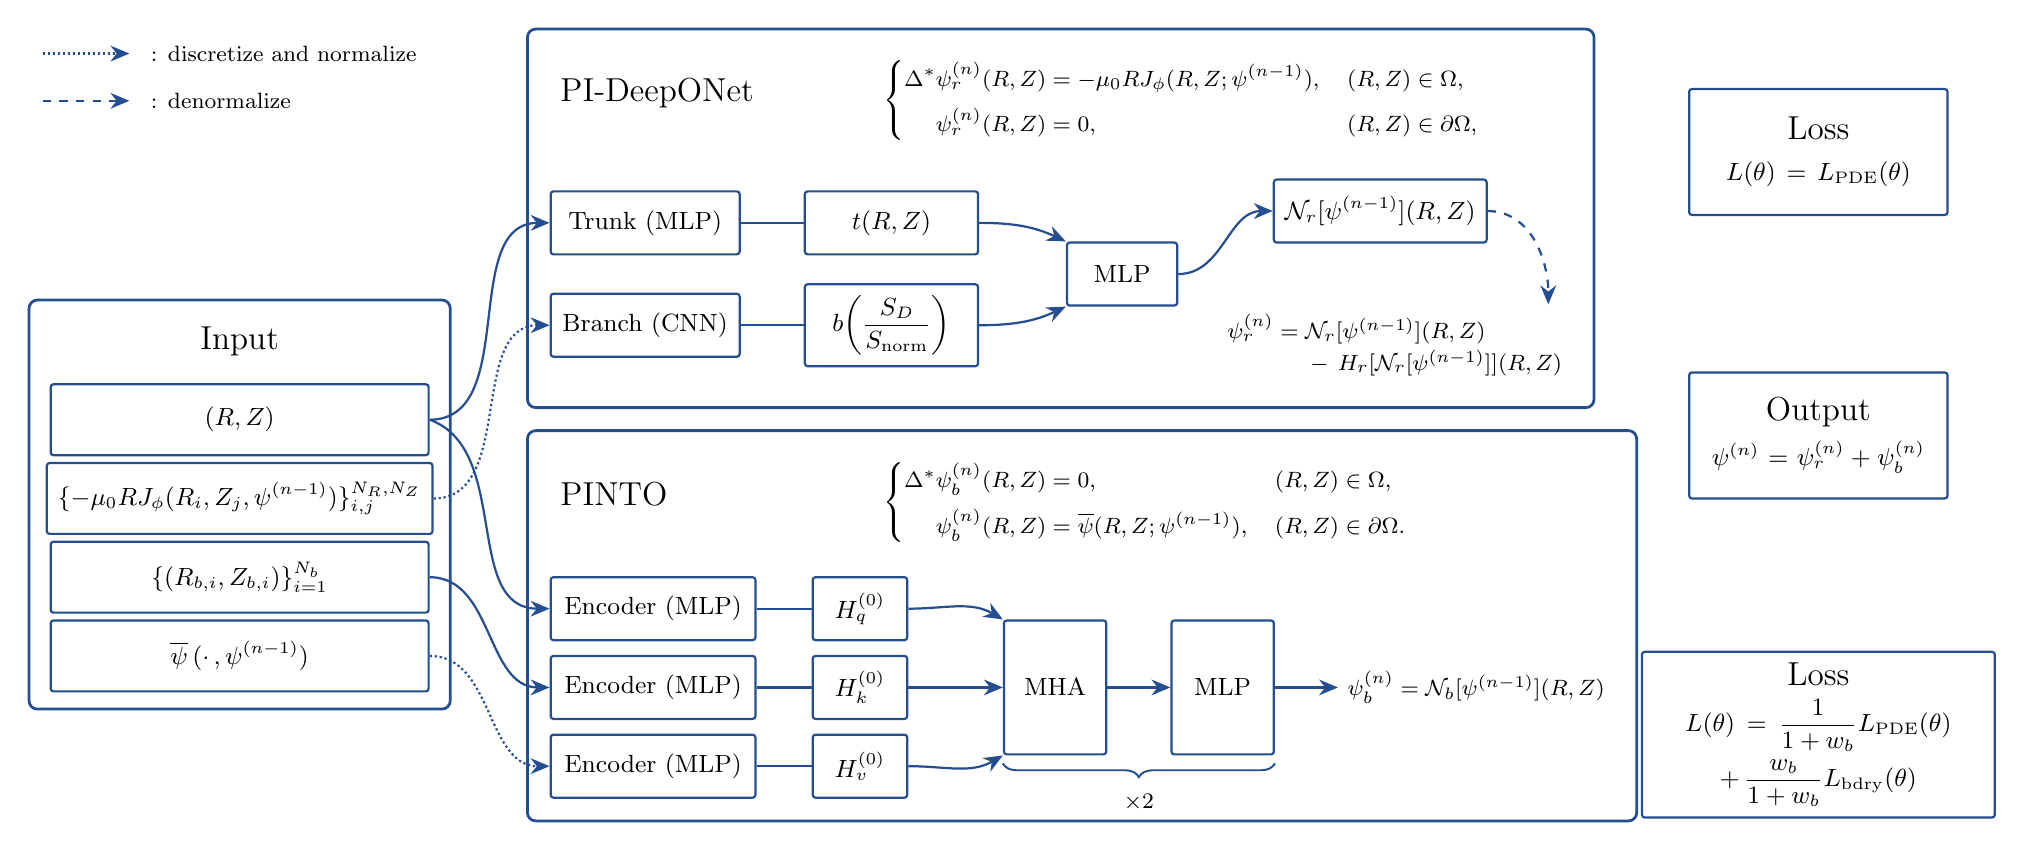
\begin{tikzpicture}[
  font=\small,
  bx/.style   ={draw=nvy, line width=.8pt, fill=white, rounded corners=1pt,
                align=center, inner sep=4pt, minimum height=8mm},
  bxi/.style  ={bx, minimum width=48mm, minimum height=9mm},   % uniform Input boxes (fit widest formula)
  small/.style={draw=nvy, line width=.8pt, fill=white, rounded corners=1pt,
                align=center, inner sep=3pt, minimum height=8mm, minimum width=12mm},
  ttl/.style  ={font=\large},
  flow/.style ={-{Stealth[length=2.4mm,width=2mm]}, draw=nvy, line width=.8pt},
  nrm/.style  ={-{Stealth[length=2.4mm,width=2mm]}, draw=nvy, line width=.8pt, densely dotted},
  dnm/.style  ={-{Stealth[length=2.4mm,width=2mm]}, draw=nvy, line width=.8pt, dashed},
  grp/.style  ={draw=nvy, line width=1pt, rounded corners=3pt, fill=white},
]

% =========================== LEGEND (top-left) ===========================
\draw[nrm] (0.05,10.2) -- (1.15,10.2);
\node[anchor=west, font=\footnotesize] at (1.3,10.2) {: discretize and normalize};
\draw[dnm] (0.05,9.6) -- (1.15,9.6);
\node[anchor=west, font=\footnotesize] at (1.3,9.6) {: denormalize};

% =========================== INPUT block ===========================
\node[ttl] (inttl) at (2.55,6.55) {Input};
\node[bxi] (inRZ)  at (2.55,5.55) {$(R,Z)$};
\node[bxi] (inJ)   at (2.55,4.55) {$\{-\mu_0 R J_\phi(R_i,Z_j,\psi^{(n-1)})\}_{i,j}^{N_R,N_Z}$};
\node[bxi] (inRb)  at (2.55,3.55) {$\{(R_{b,i},Z_{b,i})\}_{i=1}^{N_b}$};
\node[bxi] (inPsi) at (2.55,2.55) {$\overline{\psi}\,(\cdot\,,\psi^{(n-1)})$};

% =========================== PI-DeepONet inner nodes ===========================
\node[ttl, anchor=west] (dtitle) at (6.5,9.7) {PI-DeepONet};
\node[anchor=west, align=left, font=\footnotesize] (dpde) at (10.6,9.6)
  {$\left\{\begin{aligned}
     \Delta^*\psi_r^{(n)}(R,Z) &= -\mu_0 R J_\phi(R,Z;\psi^{(n-1)}), & (R,Z)&\in\Omega,\\[1pt]
     \psi_r^{(n)}(R,Z) &= 0, & (R,Z)&\in\partial\Omega,
   \end{aligned}\right.$};
\node[bx, minimum width=24mm] (trunk)  at (7.7,8.05) {Trunk (MLP)};
\node[bx, minimum width=24mm] (branch) at (7.7,6.75) {Branch (CNN)};
\node[bx, minimum width=22mm, right=8mm of trunk]  (tbox) {$t(R,Z)$};
\node[bx, minimum width=22mm, right=8mm of branch] (bbox) {$b\!\left(\dfrac{S_D}{S_{\mathrm{norm}}}\right)$};
\coordinate (dmid) at ($(tbox.east)!0.5!(bbox.east)$);
\node[bx, minimum width=14mm, right=11mm of dmid] (mlpd) {MLP};
\node[bx, right=12mm of mlpd, yshift=8mm] (nr) {$\mathcal{N}_r[\psi^{(n-1)}](R,Z)$};
\node[anchor=west, align=left, font=\footnotesize] (hardeq) at ($(mlpd.east)+(0.5,-0.9)$)
  {$\psi_r^{(n)}=\mathcal{N}_r[\psi^{(n-1)}](R,Z)$\\[2pt]
   $\hphantom{\psi_r^{(n)}=}\;-\,H_r[\mathcal{N}_r[\psi^{(n-1)}]](R,Z)$};

% =========================== PINTO inner nodes ===========================
\node[ttl, anchor=west] (ptitle) at (6.5,4.6) {PINTO};
\node[anchor=west, align=left, font=\footnotesize] (ppde) at (10.6,4.5)
  {$\left\{\begin{aligned}
     \Delta^*\psi_b^{(n)}(R,Z) &= 0, & (R,Z)&\in\Omega,\\[1pt]
     \psi_b^{(n)}(R,Z) &= \overline{\psi}(R,Z;\psi^{(n-1)}), & (R,Z)&\in\partial\Omega.
   \end{aligned}\right.$};
\node[bx, minimum width=26mm] (encq) at (7.8,3.15) {Encoder (MLP)};
\node[bx, minimum width=26mm] (enck) at (7.8,2.15) {Encoder (MLP)};
\node[bx, minimum width=26mm] (encv) at (7.8,1.15) {Encoder (MLP)};
\node[small, right=7mm of encq] (Hq) {$H_q^{(0)}$};
\node[small, right=7mm of enck] (Hk) {$H_k^{(0)}$};
\node[small, right=7mm of encv] (Hv) {$H_v^{(0)}$};
\node[bx, minimum width=13mm, minimum height=17mm, right=12mm of Hk] (mha)  {MHA};
\node[bx, minimum width=13mm, minimum height=17mm, right=8mm of mha]  (mlpp) {MLP};
\node[anchor=west, align=left, font=\footnotesize, right=8mm of mlpp] (psibeq)
  {$\psi_b^{(n)}=\mathcal{N}_b[\psi^{(n-1)}](R,Z)$};
% x2 brace under MHA + MLP
\draw[decorate, decoration={brace, amplitude=5pt, mirror}, nvy, line width=.7pt]
  ($(mha.south west)+(0,-1mm)$) -- ($(mlpp.south east)+(0,-1mm)$);
\node[font=\footnotesize] at ($(mha.south east)!0.5!(mlpp.south west)+(0,-6mm)$) {$\times 2$};

% =========================== RIGHT column ===========================
\node[bx, text width=30mm, minimum height=16mm] (losstop) at (22.6,8.95)
  {{\large Loss}\\[4pt]$L(\theta)=L_{\mathrm{PDE}}(\theta)$};
\node[bx, text width=30mm, minimum height=16mm] (output) at (22.6,5.35)
  {{\large Output}\\[4pt]$\psi^{(n)}=\psi_r^{(n)}+\psi_b^{(n)}$};
\node[bx, text width=42mm, minimum height=20mm] (lossbot) at (22.6,1.55)
  {{\large Loss}\\[4pt]$L(\theta)=\dfrac{1}{1+w_b}L_{\mathrm{PDE}}(\theta)$\\[2pt]$+\,\dfrac{w_b}{1+w_b}L_{\mathrm{bdry}}(\theta)$};

% =========================== ARROWS ===========================
% Input fan-out (solid = coords/geometry, dotted = discretize+normalize)
\draw[flow] (inRZ.east) to[out=0,in=180] (trunk.west);
\draw[nrm]  (inJ.east)  to[out=0,in=180] (branch.west);
\draw[flow] (inRZ.east) to[out=-20,in=180] (encq.west);
\draw[flow] (inRb.east) to[out=0,in=180] (enck.west);
\draw[nrm]  (inPsi.east) to[out=0,in=180] (encv.west);
% PI-DeepONet internal
\draw[nvy, line width=.8pt] (trunk) -- (tbox);
\draw[nvy, line width=.8pt] (branch) -- (bbox);
\draw[flow] (tbox.east) to[out=0,in=155] (mlpd.north west);
\draw[flow] (bbox.east) to[out=0,in=205] (mlpd.south west);
\draw[flow] (mlpd.east) to[out=0,in=180] (nr.west);
\draw[dnm]  (nr.east) to[out=0,in=90] ($(hardeq.north east)+(-0.3,0)$);
% PINTO internal
\draw[nvy, line width=.8pt] (encq) -- (Hq);
\draw[nvy, line width=.8pt] (enck) -- (Hk);
\draw[nvy, line width=.8pt] (encv) -- (Hv);
\draw[flow] (Hq.east) to[out=0,in=150] (mha.north west);
\draw[flow] (Hk.east) -- (mha.west);
\draw[flow] (Hv.east) to[out=0,in=210] (mha.south west);
\draw[flow] (mha) -- (mlpp);
\draw[flow] (mlpp.east) -- (psibeq.west);

% =========================== GROUP BOXES (background) ===========================
\begin{scope}[on background layer]
  \node[grp, fit=(inttl)(inRZ)(inJ)(inRb)(inPsi), inner sep=6pt] {};
  \node[grp, fit=(dtitle)(dpde)(trunk)(tbox)(branch)(bbox)(mlpd)(nr)(hardeq), inner sep=8pt] {};
  \node[grp, fit=(ptitle)(ppde)(encq)(enck)(encv)(Hq)(Hk)(Hv)(mha)(mlpp)(psibeq), inner sep=8pt] {};
\end{scope}

\end{tikzpicture}
\end{document}
